%%%%%%%%%%%%%%%%%%%%%%%%%%%%%%%%%%%%%%%%%%%%%%%%%%%%%%%%%%%%%%%%%%%%%%%%%%%%%%%%%%%%%%%%%%%%%%%%%%%%
% NONLINEAR THEORY 
%
% 
%%%%%%%%%%%%%%%%%%%%%%%%%%%%%%%%%%%%%%%%%%%%%%%%%%%%%%%%%%%%%%%%%%%%%%%%%%%%%%%%%%%%%%%%%%%%%%%%%%%%
\chapter{Nonlinear theory}

\section{Introduction}
In the previous chapter, we investigated the linear stability of the Lamb-Chaplygin dipole and we showed that the short-wave instability can have growth rates that are comparable to those of the zigzag instability. An important question is if both of these instabilities exist, which will dominate in the transition to turbulence? In the atmosphere and ocean, a wide range of length scales are excited, so it is expected that both the zigzag instability and the short-wave instability will be excited in nature. Understanding the evolution of these two instabilities and what role they play in the transition to turbulence is important to correctly understand the mechanisms at play in the transition to stratified turbulence. Unfortunately, as alluded to in Chapter 2, linear stability analysis can only take us so far. 

In this chapter we evolve the full nonlinear Boussinesq equations to determine how the short-wave instability evolves and what role it plays in the transition to turbulence. The importance of the zigzag instability in the breakdown and transition to turbulence has been well studied \cite{augier2012,waitesmol2008,augierbillant2011,delonclebc2008} and none of these studies have mentioned short-wavelength instabilities. In this chapter we investigate the role of the short-wave instability in the transition to turbulence. Through nonlinear simulations, we will demonstrate that the saturation level of the short-wave instability is relatively small and depends upon the aspect ratio $\delta=L_{v}/L_{h}$. Thus, for many geophysical flows, where $\delta\ll 1$, the short-wave instability does not affect the overall breakdown and transition to turbulence. 

\section{Set-up} 
To investigate the nonlinear evolution, we use a code developed by Waite (and others? first paper to use is..?). The code implements the spectral method technique discussed in Chapter 3 to solve the nonlinear Boussinesq equations. Unlike in linear stability analysis, nonlinear analysis of the Boussinesq equations is much more complicated as particular attention must be taken to ensure proper resolution of the small scales. Although we are not doing a full dynamical numerical simulation (DNS), where we would be resolving everything, the breakdown of the zigzag instability exhibits small scale turbulence which suggests that we might observe a similar result for the short-wave instability. Thus we need to choose grid sizes that approximately resolve the smallest scales, known as the Kolmogorov scale. 

The Kolmogorov scale is given by \cite{lesieur}
\begin{align}
\eta = \left(\frac{\nu^{3}}{\epsilon}\right)^{3},
\end{align}
where $\epsilon$ is the kinetic energy dissipation rate, which is commonly approximated as \cite{lindborg2006}
\begin{align}
\epsilon \sim \frac{U^{3}}{R} ,
\end{align}
where $U,R$ are the characteristic velocity and length respectively. Rewriting the Kolmogorov scale $\eta$ in terms of the Reynolds number by multiplying by the characteristic length $R$ we obtain
\begin{align}
\frac{\eta}{R} = \frac{1}{\Re^{3/4}}.
\end{align}
As discussed previously, stratified flow has two distinct directions, the horizontal and vertical and thus for our simulations, the code sets the horizontal and vertical resolutions independently, which we denote by $\Delta x$ and $\Delta z$. We want to choose the number of grid points to be such that $\Delta x \approx \Delta z \approx \eta/R$.

To focus specifically on the short-wave instability, we choose the vertical scale to be that of the short-wave instability. To illustrate, consider $Re=2000, F_{h}=0.2$ where the short-wave instability peaks at $k_{z}=20$. Here the vertical scale is 
\begin{align}
L_{v} = \frac{2\pi}{k_{z}} = \frac{2\pi}{20}.
\end{align}
Note that this vertical scale also sets the scaling for the vertical wavenumbers in the full nonlinear simulation. From our linear results, we again take $L=9$. Due to the set-up of the code, the number of grid points in every direction has to be a power of $2$. Thus let us a priori consider the number of horizontal grid points to be $N=1024$. We have that the horizontal resolution is
\begin{align}
\Delta x = \frac{L}{N} = \frac{9}{1024}\approx 0.00878,\qquad \frac{\eta}{R}\sim \frac{1}{Re^{3/4}}=0.003343,
\end{align}
and we approximately have that $\Delta x \sim \eta/R$. Even though this may be cause for concern based on our definition of the Kolmogorov scale, DNS with $L=9$ has suggested that this resolution is sufficient (cite). If choose $N=32$ grid points in the vertical, we find that $\Delta z \approx 0.00982$ which is very similar to $\Delta x$. For our timestep we choose $\Delta = 5.0\times 10^{-4}$. Each run was initialised with a random density sinusoidal perturbation with $\epsilon=0.01$. 


\section{Results}
As mentioned in the introduction, previous investigations into the transition of turbulence have focused only on the zigzag instability. In all these simulations, it is clear that the dominant instability is the zigzag instability. For example, in Waite and Smolarkiewicz \cite{waitesmol2008}, the growth rates of the zigzag instability agree with the linear theory. It is possible that these simulations were not resolving the small scales, although this does not seem likely based on the parameters given. This is because the length scale of the short-wave instability is about an order of magnitude or so smaller than that of the zigzag instability. Since these simulations were intended to study the transition to turbulence, they would be resolving, or close to resolving, the Kolmogorov scale, which is much smaller than the short-wave instability. Hence it is unlikely a resolution issue. Instead, it could be the case that the short-wave instability is present but saturates out and does not contribute significantly to the transition to turbulence. We explore this option here. 

Consider the following scaling argument and results due to Ngan, et al.\cite{ngan2005}. They were interested in three-dimensionalisation of a two-dimensional flow, specifically the case of quasi-two dimensional turbulence, which is an in-between case between 2D turbulence and 3D turbulence. They considered this as they were interested in geophysical flows which exhibit small aspect ratios, $\delta=0.01-0.1$ \cite{ngan2005}. As we have seen, stratified turbulence tends to have a small aspect ratio and, as discussed in Chapter 2, exhibits characteristics of quasi-geophysical flow which shares characteristics with a two-dimesional flow being three-dimensionalised. However, it is important to note that Ngan et al.\cite{ngan2005} did not consider stratification and they were only focusing on the unstratified case of turbulence with small aspect ratios. 

To investigate this three-dimensionalisation, in their numerical experiments they took fully developed 2D turbulence and subjected it to a 3D perturbation. They then measured the saturation level of this 3D perturbation. The saturation level is defined to be
\begin{align}
\text{saturation} = \frac{u}{U}\bigg|_{t=sat}, \label{ngan_scale}
\end{align}
where the ratio between the 3D velocity $u$ and the 2D velocity $U$ are evaluated at the saturation time. The saturation time is the time at which the time series of the 3D velocity levels off or saturates. They found, numerically, that this saturation level depended linearly on the aspect ratio $\delta$, up to a certain aspect ratio, $\delta=0.5$. Beyond $\delta=0.5$ the numerical simulations could no longer be considered quasi-two dimensional. 

To explain this result, Ngan et al. considered a simple scaling argument \cite{ngan2004,ngan2005}. Initially the time scales of the 2D base flow is long compared to that of the 3D perturbation flow. However once the 3D perturbation settles down and saturates, its timescale becomes similar to that of the 2D flow.  Consider the following timescales for these flows \cite{ngan2005} as
\begin{align}
T_{2D} = \frac{U}{L},\qquad T_{3D} =\frac{u}{H}
\end{align}
where $U$ is the characteristic velocity of the 2D flow at saturation and $u$ is the characteristic velocity of the 3D flow at saturation. At saturation $T_{2D}\sim T_{3D}$ and thus we have that 
\begin{align}
\frac{U}{L}\sim\frac{u}{H} \Rightarrow \frac{u}{U} \sim \frac{H}{L} = \delta,
\end{align}
which is the result they confirmed numerically. 

Motivated by this result, we consider the saturation levels of the short-wave instability for $Re=2000,5000$ and $F_{h}=0.2$. These two cases were chosen as they both had short-wave instability growth rates similar to that of the zigzag peak. Higher $Re$ could not be explored due to resolution issues, as alluded to in the previous section. We differ from Ngan et al.\cite{ngan2005} in that we instead consider the energy instead of the velocity.\begin{align}
\text{saturation} = \frac{E_{2D}}{E_{3D}}\bigg|_{t=sat}.
\end{align}
Additionally, unlike Ngan et al.\cite{ngan2005} we also have potential energy.  

To compute the saturation level, the code allows for two possibilities. The first is to compute the kinetic and potential energy directly from the definition, as discussed in Chapter 3. The other is to compute the 2D and 3D energy directly from the vertical spectrum. 

In the first case, we compute the kinetic and potential energies and associate the 2D flow with the kinetic energy and the 3D perturbation with the potential energy. This is justifiable by realising that the basic state, the Lamb-Chaplygin dipole, is initially kinetic energy only and thus the potential energy is coming strictly from the 3D perturbation. 

The other method is to determine the 2D and 3D energy directly summing the vertical spectrum. In our simulations, the vertical spectrum had wavenumbers $k_{z}=0,1,\ldots,11$. Recall that here $k_{z}$ has been non-dimensionalised with the short-wave instability and thus $k_{z}=1$ corresponds to the wavelength of the short-wave instability. $k_{z}=0$ corresponds to the 2D dimensional energy and the sum of the remaining wavenumbers corresponds to the 3D energy. 

Both methods were used to compute the saturation level and it was found that the results using the kinetic and potential energy were better than directly computing the 2D and 3D energy from the vertical spectrum. Fig.~\ref{sat_energy} demonstrates the results for $Re=5000, F_{h}=0.2, k_{z}=40$. As can be observed in the Figure, the kinetic (2D) energy from both methods are very similar and nearly indistinguishable. The big difference is for the potential (3D) energy. The spectrum method (dashed-blue) is more jagged (?) and the saturation level is less well defined. The direct computation of the energy (black) is smoother, although still has bumps, but the saturation level is approximately constant. For this reason, we choose to use the direct computation of the energy. Despite the differences, both curves have the same saturation time, roughly $T=20$. 
\begin{figure}
\begin{center}
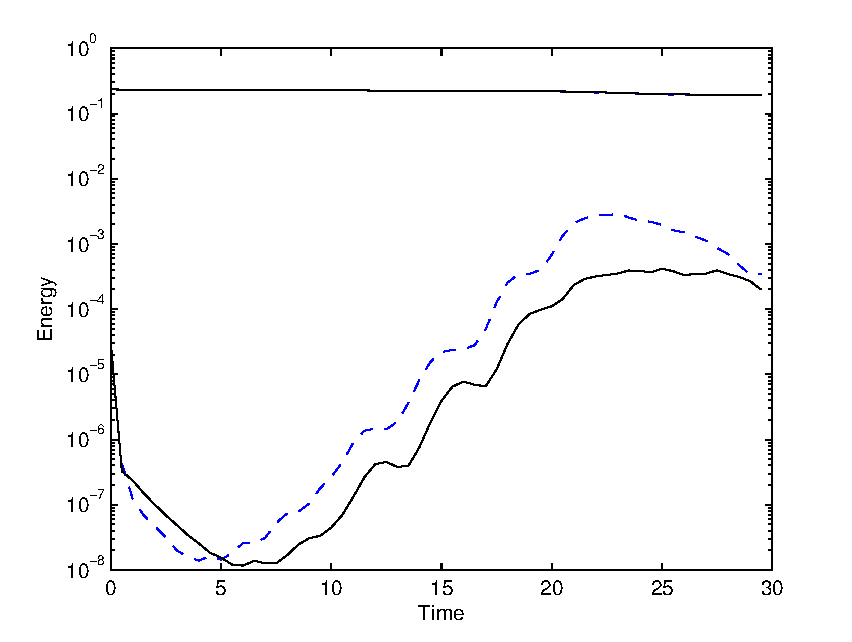
\includegraphics[width=\textwidth]{sat_eg_re5000_fh02}
\caption{Time series demonstrating the two ways of computing the energy for $Re=5000, F_{h}=0.2, k_{z}=40$. The dashed blue curves correspond to computing the energy through the vertical spectrum and the solid black curves correspond to the computing the energy directly from the fields. The top line corresponds to kinetic (2D) energy and the bottom lines correspond to potential (3D) energy.}
\label{sat_energy}
\end{center}
\end{figure}

However computing the energy from the vertical spectrum does allow for the contributions due to each wavenumber. Fig.~\ref{other_kz} demonstrates this for previous parameters. Here we can explicitly see which wavenumbers are contributing to the total 3D energy. For almost the entire simulation, the $k_{z}=1$ wavenumber dominates, as the total sum of the wavenumbers is obscured by $k_{z}=1$. However at around the saturation time $T=20$, $k_{z}=2$ appears to be contributing as the total 3D energy is a little above $k_{z}=1$. This lasts for about $5$ time units before diffusion begins to rapidly diffuse out the smaller scales, which is especially evident in the highest wavenumbers. 
\begin{figure}
\begin{center}
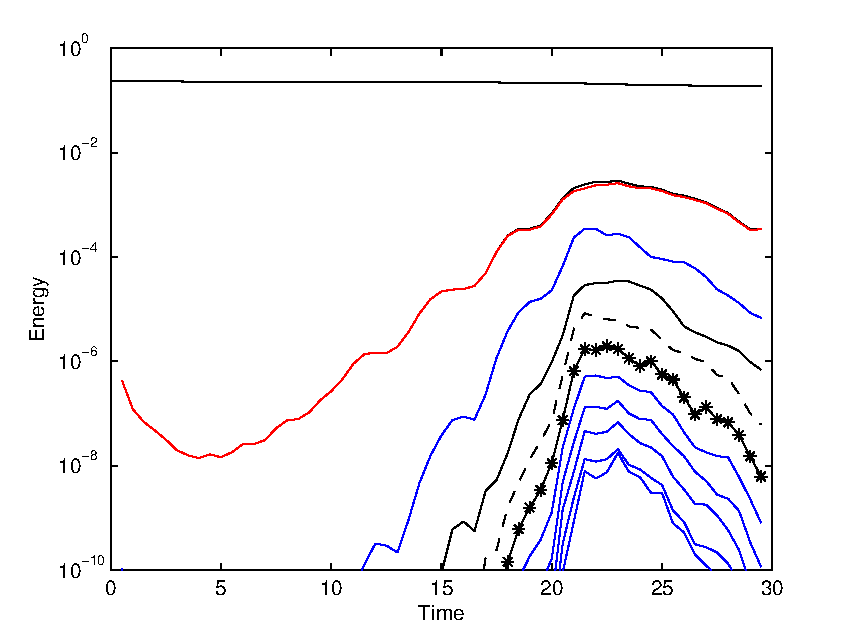
\includegraphics[width=\textwidth]{other_kz}
\caption{Time series for the energy computing from the vertical spectrum $Re=5000, F_{h}=0.2, k_{z}=40$ for different vertical wavenumbers. The top black curve corresponds to $k_{z}=0$ and is the kinetic energy. In order from top to bottom: red curve is $k_{z}=1$, blue curve is $k_{z}=2$, black curve is $k_{z}=3$, dashed black is $k_{z}=4$, star is $k_{z}=5$, and so on. The black curve that is obscured by $k_{z}=1$ is the sum of all the nonzero vertical wavenumbers.}
\label{other_kz}
\end{center}
\end{figure}

To determine the saturation level as a function of $\delta$, we investigated a range of $k_{z}$ around the short-wave instabilities for $Re=2000,5000, F_{h}=0.2$. Fig.~\ref{re2000sat} is the case of $Re=2000$. The saturation levels follow an increasing trend which agrees with Ngan et al.\cite{ngan2005}: as the aspect ratio is increased, the saturation level increases. Using a least-squares fit we find that the best fit curve is $3.02$ and have plotted a reference curve of slope $3$. Fig.~\ref{re5000sat} is the case of $Re=5000$. Again, the trend of saturation level with increasing aspect ratio is observed here. Using a least-squares fit we find that the best fit curve is $3.16$ and a reference curve of slope $3$ is plotted. At this higher Reynolds number, it was observed that although the saturation was clear, the actual time to choose to evaluate the saturation ratio was not well defined. In Fig.~\ref{sat_energy} although the saturation level here is fairly flat, there is still a bit of variation in the saturation level. In some cases this variation was more pronounced so defining where to evaluate the saturation ratio was not well defined. For consistency, the first maximum after $T=20$ time units was chosen. 

\begin{figure}
\begin{center}
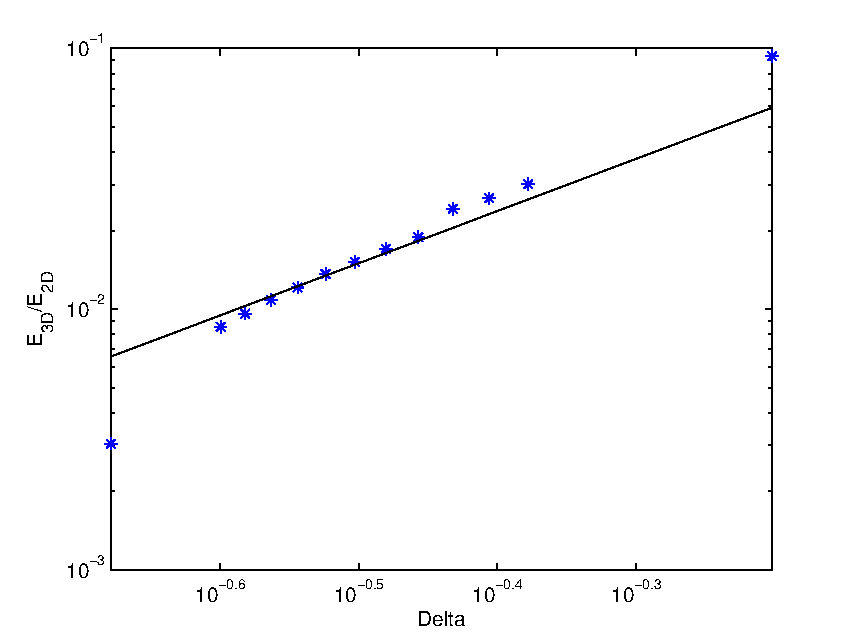
\includegraphics[width=\textwidth]{re2000_fh02_saturations} 
\caption{Saturation levels for a range of aspect ratios $\delta$ for $Re=2000$ and $F_{h}=0.2$. The curve has slope $3$.}
\label{re2000sat}
\end{center}
\end{figure}
\begin{figure}
\begin{center}
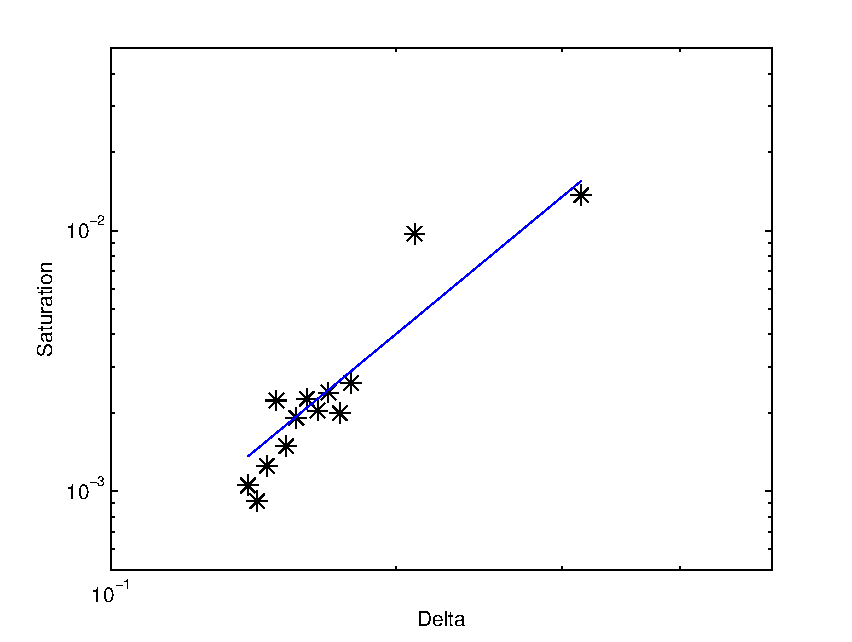
\includegraphics[width=\textwidth]{re5000_fh02_saturation_levels} 
\caption{Saturation levels for a range of aspect ratios $\delta$ for $Re=5000$ and $F_{h}=0.2$. The curve has slope $3$. }
\label{re5000sat}
\end{center}
\end{figure} 
From these two curves it suggests that the saturation level of the short-wave instability is given by
\begin{align}
\frac{E_{2D}}{E_{3D}}\bigg|_{t=sat} \sim \delta^{3},
\end{align}
which suggests that as the aspect ratio decreases, the saturation level decreases. From the linear theory, the short-wave instability was found to scale as $k_{z}\sim F_{h}^{-1/5}Re^{2/5}$ or $k_{z}'\sim F_{h}^{-1/5}Re^{2/5}/R$ in dimensional units. Then the aspect ratio scales as $\delta \sim F_{h}^{1/5}Re^{-2/5}$ and hence the saturation level is 
\begin{align}
\frac{E_{2D}}{E_{3D}}\bigg|_{t=sat} \sim (2\pi)^{3}F_{h}^{3/5}Re^{-6/5}.
\end{align}
Plugging in $Re=5000$ and $F_{h}=0.2$ yields a ratio on the order of $10^{-3}$ which agrees with Fig.~\ref{sat_energy}. For $F_{h}\ll 1$ and $Re\gg 1$ this ratio is $\ll 1$. Thus given that the short-wave instability seems to saturate at a relatively low level, we should not expect the short-wave instability to play a significant role in the evolution of the Lamb-Chaplygin dipole's transition to turbulence. 

This scaling for the saturation level differs from that of Ngan et al.\cite{ngan2005}. If we square Eq. (\ref{ngan_scale}) we obtain 
\begin{align}
\frac{u^{2}}{U^{2}} =\frac{KE_{3D}}{KE_{2D}}\sim \delta^{2},
\end{align}
which suggests that the saturation level will square quadratically instead of cubically. It is clear that their simple dimensional argument breaks down when stratification occurs, but this is not too surprising since the origins of their argument \cite{ngan2004} is based on a ``pressureless" argument where 
\begin{align}
\frac{|\nabla_{h}p|}{|\bm{u}\nabla\bm{U}|}= \mathcal{O}(\delta^{2}).
\end{align}
Using our scaling from Chapter 4, we would find, with $\rho_{0}=1$ following \cite{ngan2004}
\begin{align}
\frac{|\nabla_{h}p|}{|\bm{u}\nabla\bm{U}|}= \mathcal{O}(\delta^{-1}),
\end{align}
which is very different. Thus, we cannot use their scaling argument here. However, the similarities in results does suggest that such a dimensional argument might be possible.

Fig.~\ref{full_structure} is the vertical vorticity at three times, $T=15,20,25$. Recall that $T=20$ is the saturation time. Just before, $T=15$, the saturation the structure of the dipole does not exhibit any small-scale features. However at $T=20$, the saturation time, the dipole exhibits many small-scale features but by $T=25$ they have potentially been diffused out and the structure of the dipole has similar structure to itself before saturation, albeit with the two cores of the dipole more homogeneous in vorticity. The structure suggests that the saturation time is important as the dipole is undergoing some sort of transition, but as we saw, this transition is short lived as $5$ time units later, small-scale behaviour has potentially diffused out and there is no suggestion that the system will transition to turbulence. Indeed, this result reaffirms that the gridspace is sufficient enough to resolve the nonlinear evolution. Since this plot does not exhibit any features of turbulence, needing to resolve the Kolmogorov scale is not required. 
\begin{figure}
\begin{center}
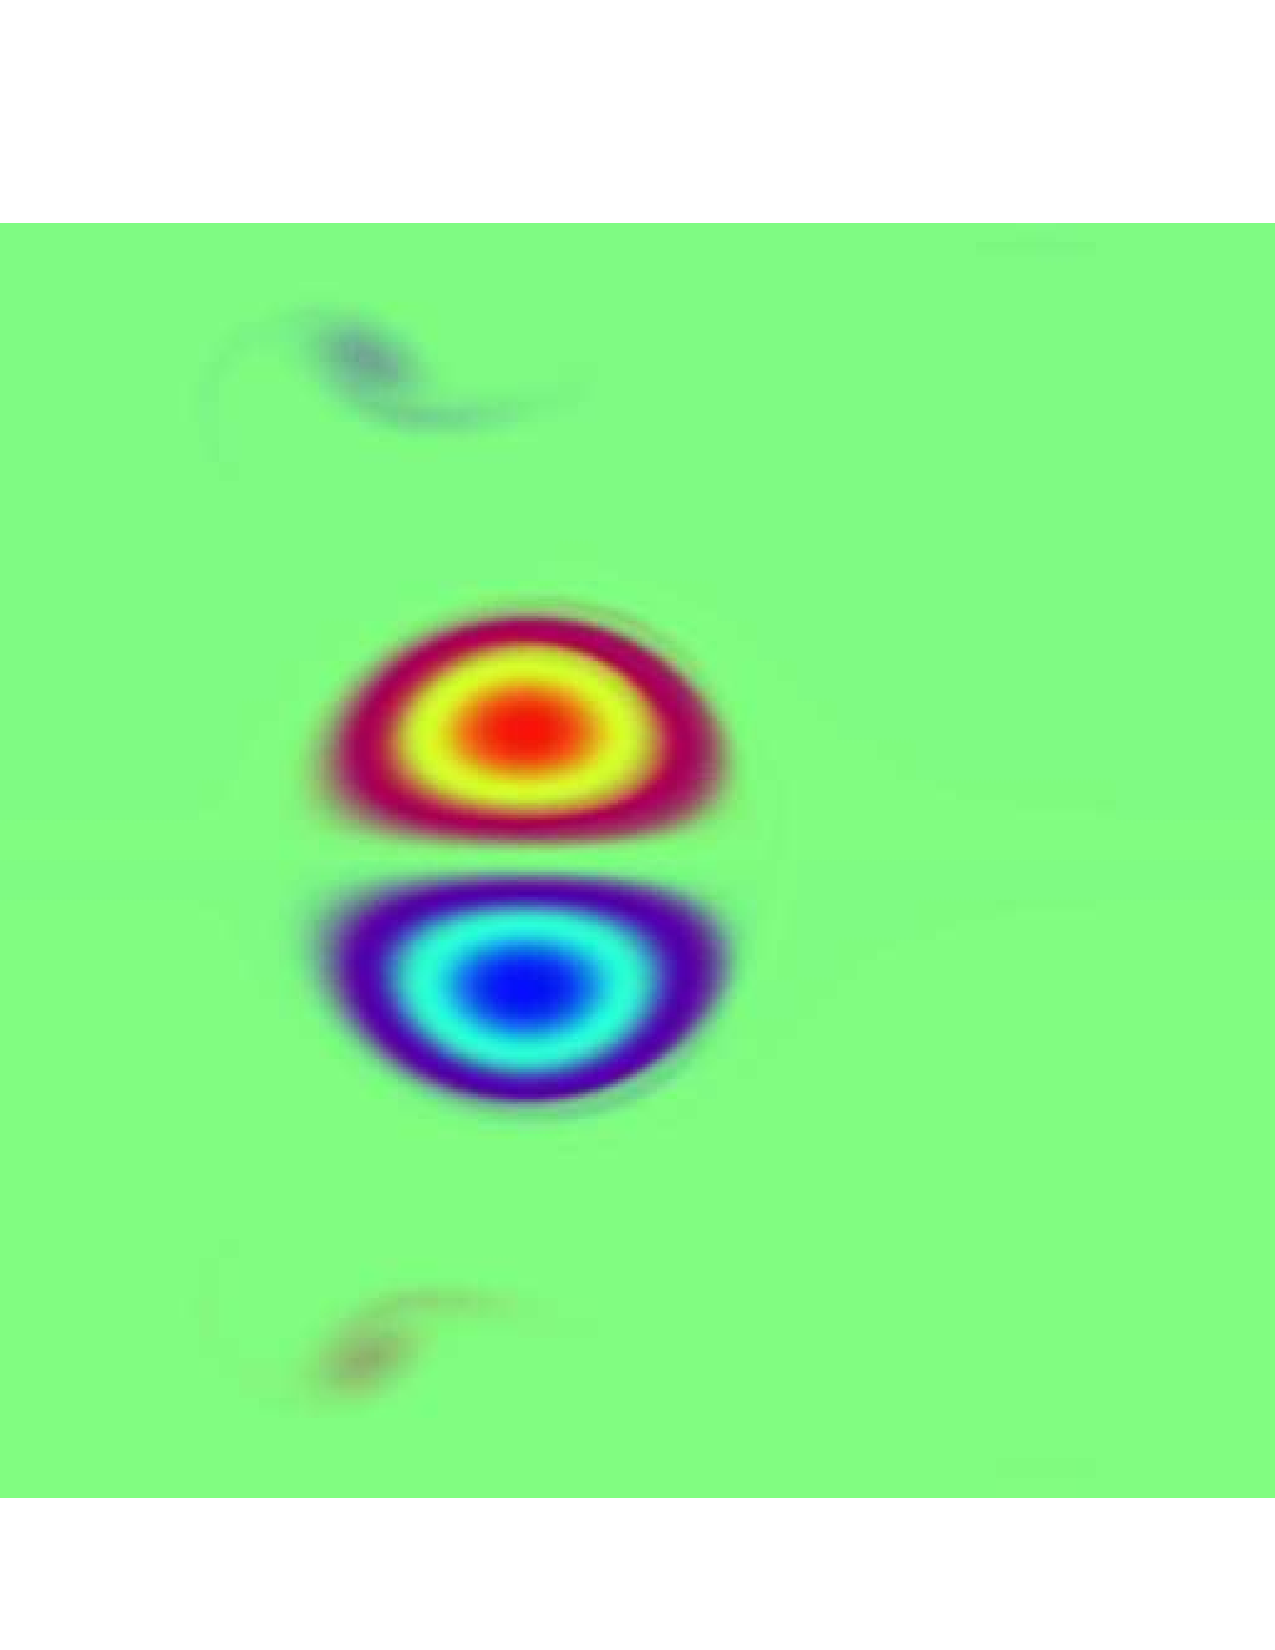
\includegraphics[width=0.4\textwidth]{struc_3}
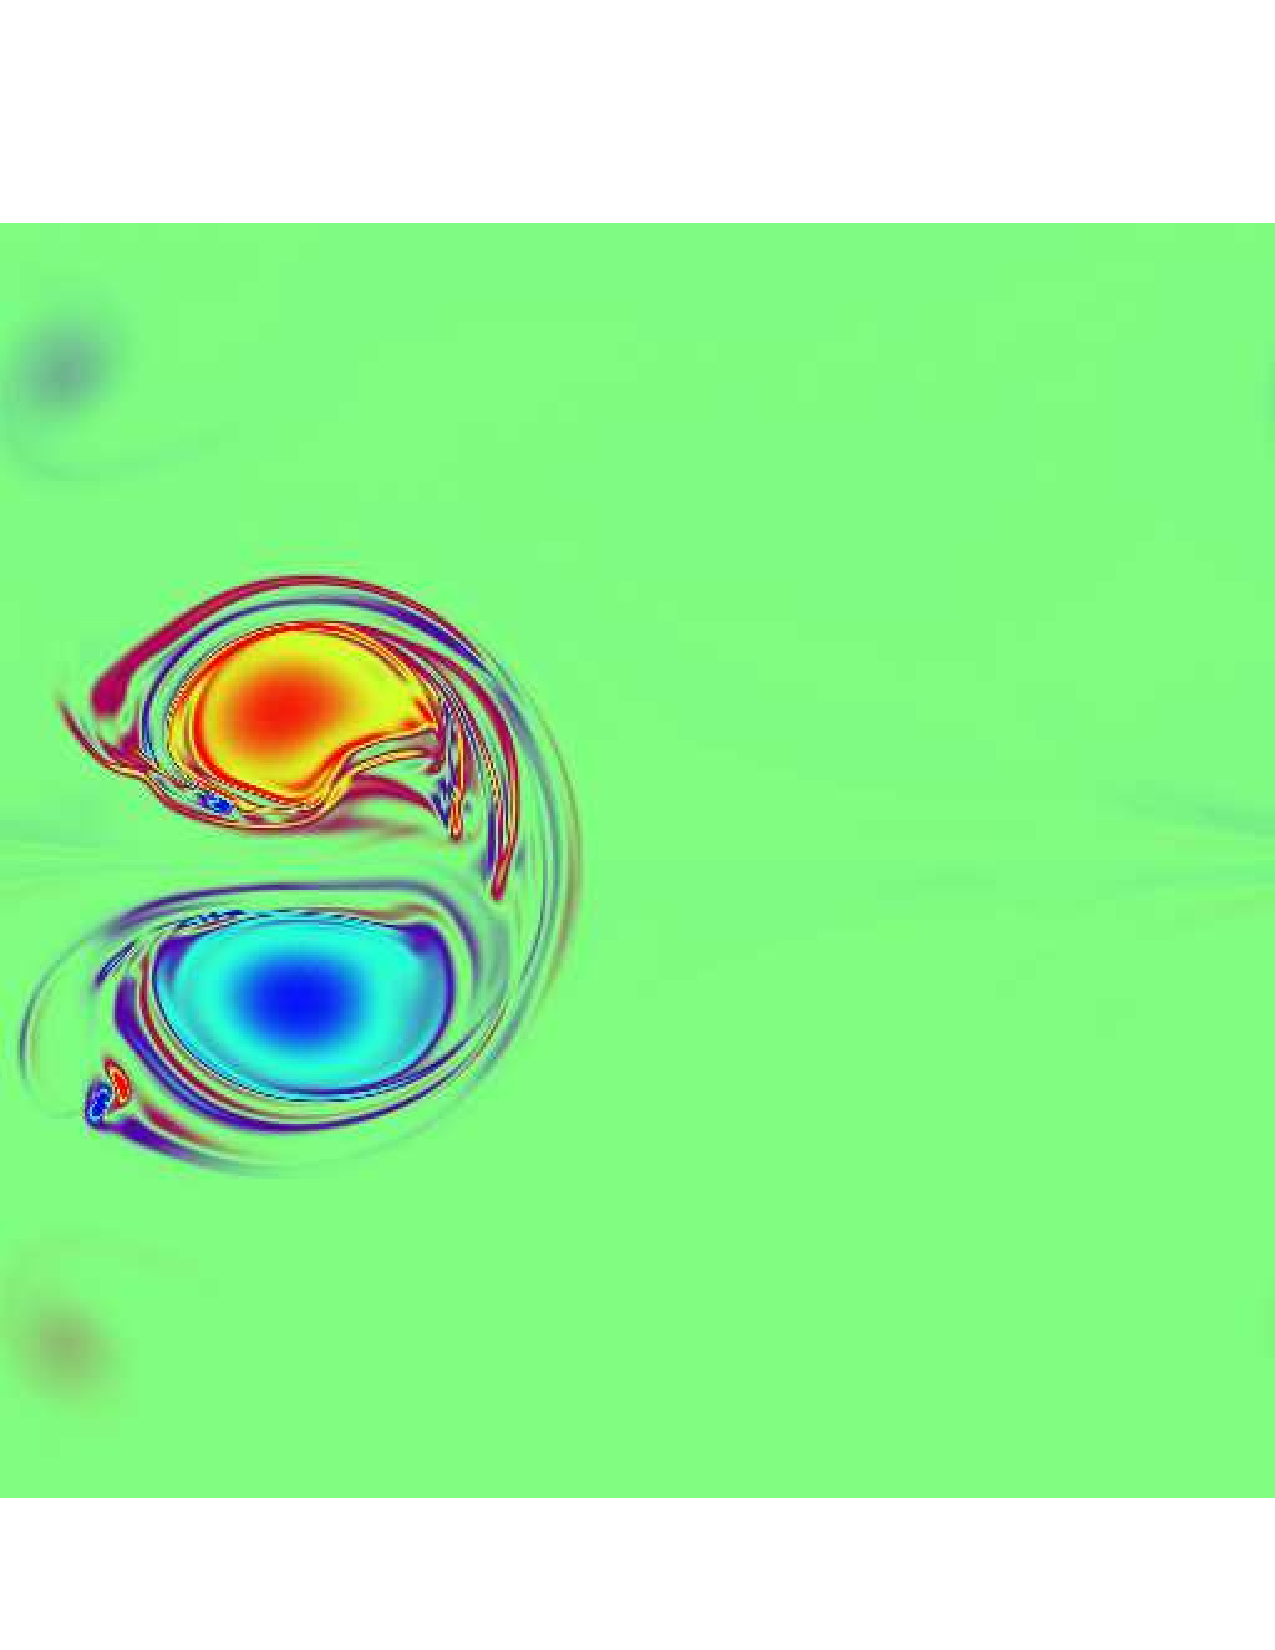
\includegraphics[width=0.4\textwidth]{struc_4}
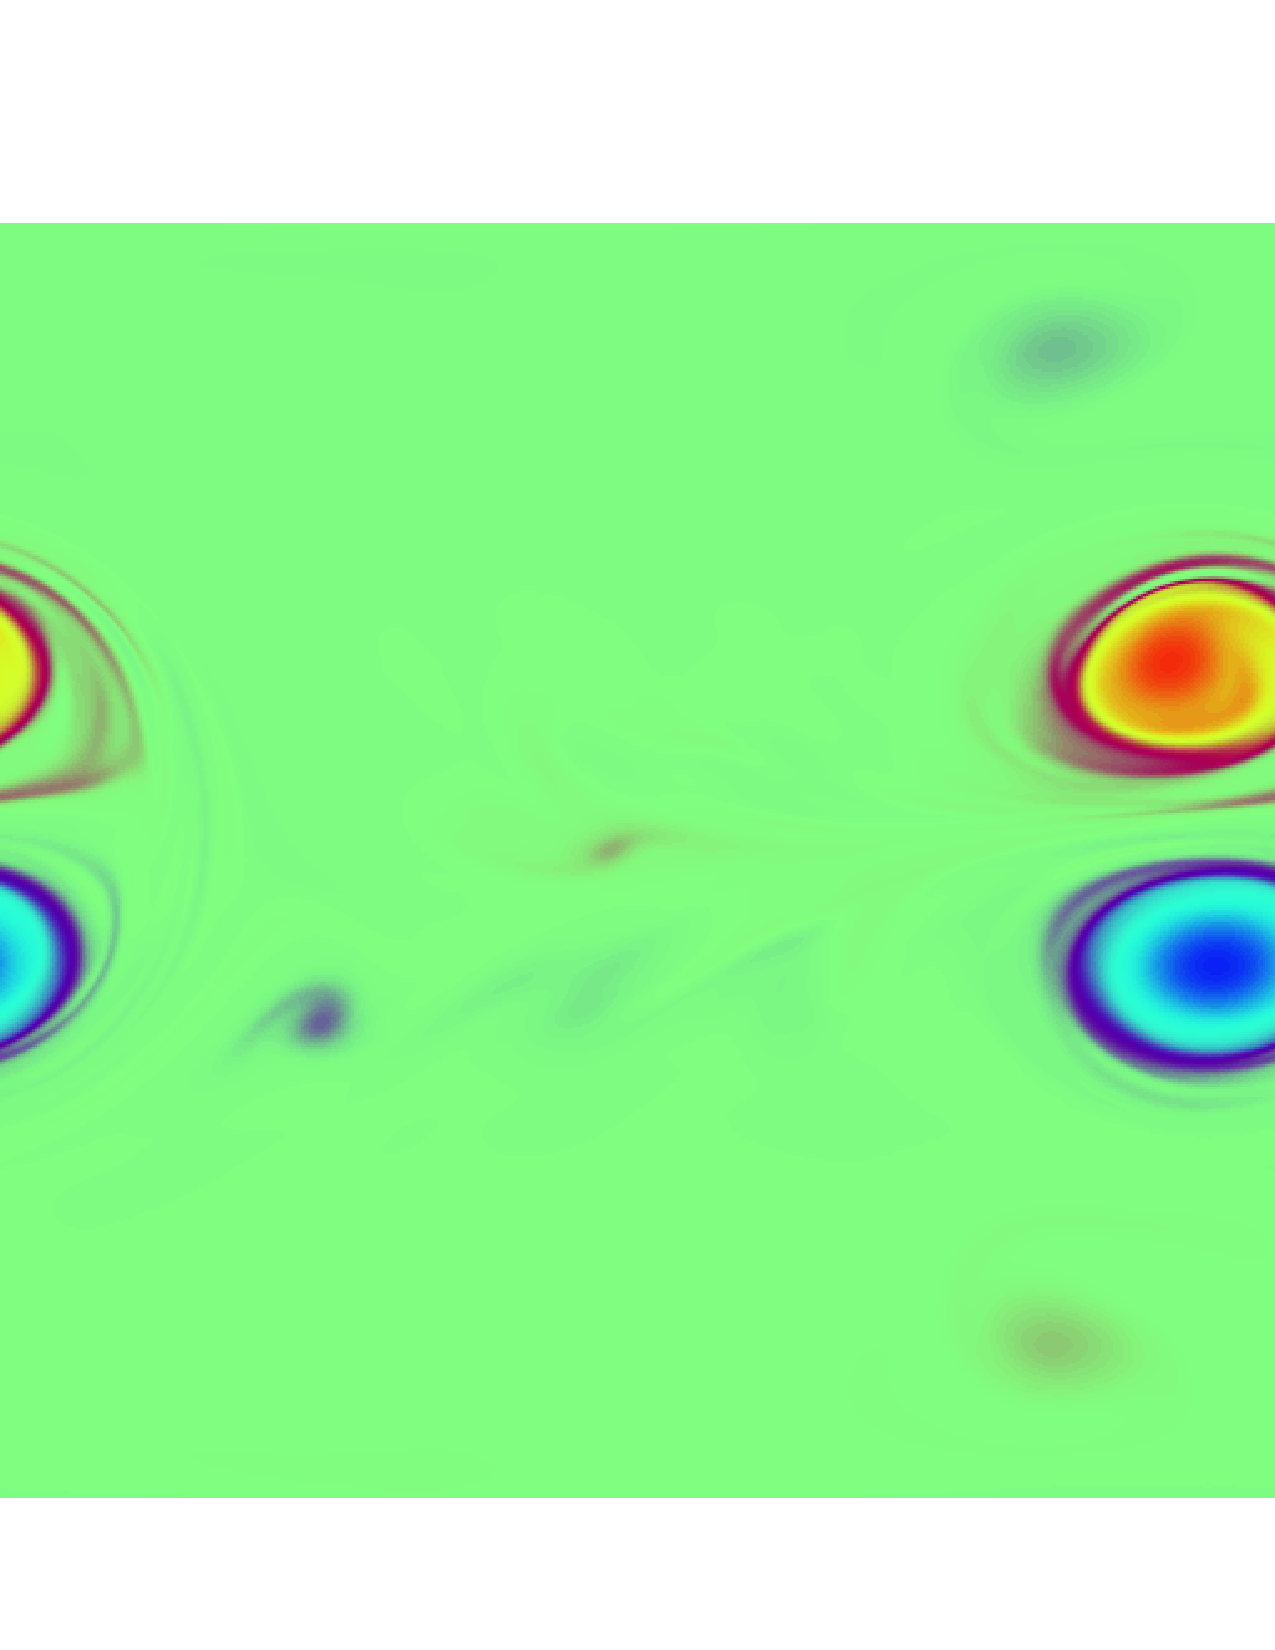
\includegraphics[width=0.4\textwidth]{struc_5}
\caption{Evolution of the vertical vorticity for $Re=5000, F_{h}=0.2, k_{z}=40$ for $T=15$ (top right), $T=20$ (top left), $T=25$ (bottom). Red corresponds to maximum vorticity and blue corresponds to minimum vorticity.}
\label{full_structure}
\end{center}
\end{figure}

We now examine the growth rate of the linear theory and that of the nonlinear theory. In comparing the linear theory with the nonlinear theory, there is a problem with what defines the linear regime of the nonlinear simulation. If we examine Fig.~\ref{sat_energy}, the growth of the potential energy between $T=5$ and $T=20$, it is very difficult to justify approximating this growth rate as linear. For most of the cases of $Re=5000$ and $F_{h}=0.2$, we were unable to determine a consistent way to determine the growth rate of the perturbation and thus we have not included the results for this simulation. Fig.~\ref{growth_rates_nonlinear} illustrates the results for the linear and nonlinear theories for $Re=2000$ and $F_{h}=0.2$. Here the nonlinear results are greater than those of the linear theory, however the curve still follows the linear theory curve. Again, the issue of the growth in the potential energy not being perfectly linear could contribute to this discrepancy of $8\%-40\%$. 

\begin{figure}
\begin{center}
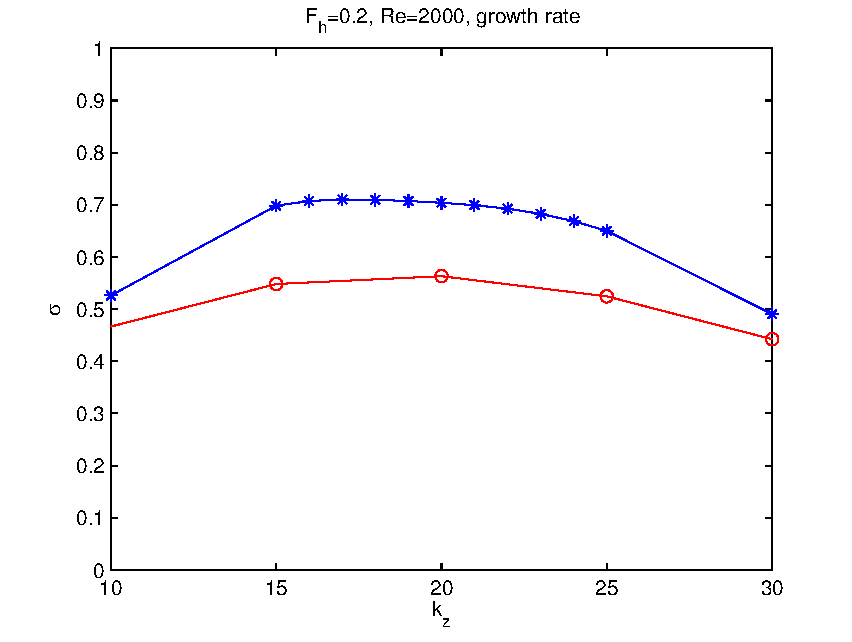
\includegraphics[width=\textwidth]{re2000_fh02_growth_rates} 
\caption{Growth rate for $Re=5000$ and $F_{h}=0.2$ with the linear results (red) and the nonlinear results (blue). Note we have not scaled by $F_{h}$ unlike the results in Chapter 3.}
\label{growth_rates_nonlinear}
\end{center}
\end{figure}

We conclude with a brief discussion of the consistency of the results. To ensure our results were consistent, we ran another simulation with $L=5$ and $N=64$ for the vertical wavenumber. This increase in the number of grid points in the vertical is to ensure that $\Delta x \sim \Delta z$ because decreasing $L$ decreases $\Delta x$ so $\Delta z$ must do so similarly. The results are plotted in Fig.~\ref{test_energy}. As can be observed, the overall amount of energy in the system is higher with $L=5$ because the domain is smaller and hence the dipole takes up a greater percentage of available grid points. Calculating the saturation level, here taken to be the maximum of the potential energy, yields a difference of $2\%$ between $L=5$ and $L=9$. In calculating the growth rate there is a difference of $8\%$. Thus if we increase the resolution, we will obtain similar results. Due to the way the code was set-up, using $L=5$ was not feasible to use as doubling the number of vertical grid points approximately doubled the simulation time. 
\begin{figure}
\begin{center}
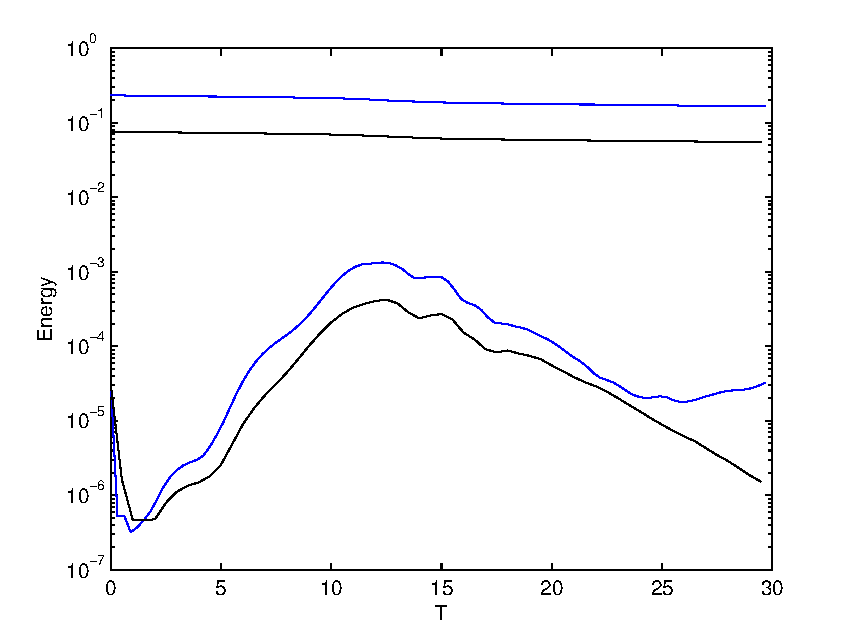
\includegraphics[width=\textwidth]{energy_test}
\caption{Time series of the potential energy (bottom curves) and kinetic energy (top curves) for $L=5$ (blue) and $L=9$ (black). Here $Re=2000, F_{h}=0.2,k_{z}=20$.}
\label{test_energy}
\end{center}
\end{figure}





